\documentclass{acm_proc_article-sp}	
%\bibliographystyle{apalike} %% <---
\pagenumbering{arabic}
\usepackage{url}
\usepackage{enumitem}
\usepackage{url}
%\usepackage{hyperref}
% nicer tables: booktab
\usepackage{booktabs}
\setlength{\abovetopsep}{1ex}
\setlength{\textfloatsep}{0.3cm}

% remove copyright stuff
\makeatletter
\def\@copyrightspace{\relax}
\makeatother


\begin{document}

%\title{Designing and Measuring Game Feel in\\2D Platforming Games}


  \title{%
  %Measuring Game Feel And The Impact of Control\\
  %Measuring the Impact of Player Control on Game Feel\\
  %Measuring the Impact of Modulating Control on Game Feel
  Measuring How Game Feel Is Influenced by\\the Player Avatar's Acceleration and Deceleration\\
  \large Using a 2D Platformer to Describe Players' Perception of Controls in Videogames}





\numberofauthors{1}
\author{
\alignauthor
Gustav Dahl\\
       \affaddr{Aalborg University, Denmark}\\
       \email{gdahl11@student.aau.dk}
}

\maketitle

\begin{abstract}
The feel of videogames is important, but not very well understood. Game feel is an integral part of game design and is the moment-to-moment sensation of control in games. Since it is something the player is constantly experiencing, it is important to be able to define when a game feels `twitchy' or `floaty'. There is a lack of vocabulary for designers and players to be able to talk about game feel. This paper sets out to investigate what words players use to describe the feel of a game, as well as what kind of parameters yield these words. This is achieved using a 2D platforming game in which the response of the player avatar motion is modulated. The velocity of the avatar changes between rounds, so that the acceleration and deceleration is either quick or slow. This changes the feel of the game. Players were asked to describe these feelings, as well as rate them in categories such as how `fluid', `floaty' and `responsive' the game felt. It was found that players have a hard time distinguishing between the velocities when the response time is below 250 ms. However, when the acceleration and deceleration took more than 250 ms, players reported the controls to feel very unresponsive and stiff. It was found that the players react more strongly to slow acceleration than deceleration. Whether these findings apply to other game genres is yet to be investigated.

\end{abstract}

% A category with the (minimum) three required fields
%\category{H.4}{Information Systems Applications}{Miscellaneous}
%A category including the fourth, optional field follows...
%\category{D.2.8}{Software Engineering}{Metrics}[complexity measures, performance measures]

%\terms{Experimentation}

\keywords{Game design, game feel, game development, perception} % NOT required for Proceedings

\section{Introduction}
Game design is a difficult discipline that typically requires many years of experience to get right. An important aspect of game design is \textit{game feel}, i.e., the sensation of control in a videogame, as described by Swink \cite{swink}. Game feel is the extension of the player's senses. It's caused by a constant feedback loop between player and system. At its core, game feel can be described as the pure enjoyment of moving a player avatar around on the screen. Game feel happens from the moment players form an intention in their heads and press a button, to when they see the response on the screen (e.g., the avatar jumping). Whenever players interact with a game, they are exposed to the feel of that game. This means that the feel can make or break the player experience.

The current state of designing game feel is that of an iterative process wherein designers have to carefully consider and tweak every aspect to get the game feeling ``right". This process often relies on the gut feeling of the game designers and lots of tweaking and testing \cite{meatboy1, juicyBeast, platformer_controls}.

Even though game feel is usually based on the simulation of a virtual world, it can still be related to the physical world. Every object in the physical world has properties that define their unique feel, e.g., their textures, shapes and interactive properties. While a bowling ball feels massive and heavy, a knife feels sharp, pointy and thin. When it comes to games, designers and players don't have the required vocabulary to talk about these characteristics. Players might describe a certain game feeling `floaty', `twitchy' or `responsive', but there are no de facto terms that can be used to talk about a specific game feel. It is uncertain when a game goes from being `twitchy' to `floaty'. Game feel consists of many elements, such as graphical presentation, physical simulations, sounds, player controls, input device, camera movement, level design, etc. 

While game feel might be a loose concept, there is still the notion of responsiveness. Game programmer West argued that \textit{``the `feel' of a game is, in large part, described in terms of how responsive it is. Very often a game will be described as `laggy' or `sluggish', and by contrast other games will be `tight' or `fast'."} \cite{measure_lag} 

To get a better understanding of how players perceive and talk about game feel, this paper sets out to investigate two questions: A) What words players use to describe the feel of a game, and B) Which parameters yield those specific descriptions. This study is based on a simple 2D platforming game where players control a rolling ball with the keyboard. The acceleration and deceleration of the player's avatar change, separately, between rounds. To test the influence of changing these parameters, an experiment was conducted by uploading the game to the Internet. Participants had to play the same game four times, where each round changed the acceleration and deceleration. Between the rounds, they were asked to describe the feel of the controls in their own words, as well as rate it based on pre-defined terms such as how `twitchy', `fluid' and `stiff' the game felt. 274 players participated in the experiment.
%This paper describes the background, setup and findings of the experiment. Section \ref{stateOfTheArt} describes the state of the art within the area of game feel, as well as related topics. Section \ref{design} presents a short description of the game that was developed for this project. Section \ref{experimentalDesign} describes the thoughts behind the experimental design. Section \ref{data} provides an analysis of the collected data, and, lastly, Section \ref{discussion} discusses and concludes upon this data.

\section{State of the Art} \label{stateOfTheArt}
%Section \ref{define_GF} provides a definition of game feel and describes other relevant topics. Section \ref{colour} looks at a study about how people describe colours. This study has been used as inspiration for conducting the experiment about how people describe game feel. Section \ref{marioLevel} reviews a study that built a set of questionnaires directly into a game, which was then put online.

%This paper sets out to investigate one of these aspects, namely the influence of movement controls in 2D platforming games.

%\subsection{Defining Game Feel} \label{define_GF}
Game feel is a relatively unexplored research area. The primary literature on the topic is the book \textit{Game Feel: A Game Designer's Guide to Virtual Sensation} by Swink \cite{swink}. `Feel' is not meant in a thematic nor emotional/physical sense. Instead it's the kinesthetic sense of manipulating a virtual object --- the sensation of real-time control in a videogame. Swink provided the following definition of game feel: \textit{real-time control of virtual objects in a simulated space, with interactions emphasized by polish} \cite{swink}.
%These elements will be discussed further in the following sections.
%\subsection{Reacting to Player Input}

An important aspect of game feel is controlling virtual objects and how responsive these controls are. Normoyle and J\"{o}rg conducted a study to investigate the relationship between the naturalness of motion (e.g., in the form of realistic and adaptive 3D animations) versus responsiveness (the game reacts instantly to the player's input, regardless of which phase the animation is in) \cite{normoyle_trade-offs_2014}. Developers typically need to make trade-offs between naturalness and promptness when designing and implementing player controls and animations. This can affect the player's overall sense of control, enjoyment, satisfaction and performance. To test this, Normoyle and J\"{o}rg  created a 3D game with varying degrees of animation blendings. The more natural the animations blend together when moving, the less responsive the character is (e.g., the player has to wait for the virtual character to complete a ``turn-around" animation). While playing, 67 participants tried the different animation types.  Data was collected by logging the participants' performance in the game, as well as asking them about their experiences via a post-questionnaire. Normoyle and J\"{o}rg concluded that one should always prioritize responsiveness, since low responsiveness negatively affects players' perceived ease of use, as well as their objective performances \cite{normoyle_trade-offs_2014}.

%This knowledge can be tied into the Model Human Processor \cite{card1986model, swink}, implying that games should respond to the player's input within 240 milliseconds in order to appear instant. Swink described feedback happening within 100 milliseconds as being `instant' and within 100-240 milliseconds as being `sluggish'. This perception is gradual, and if there is a delay of more than 240 milliseconds, the sense of real-time control might break \cite{swink}.

How quickly a game reacts to player input is important. One way to measure this latency is provided by West \cite{measure_lag}. He presented ways to measure response lag and how it can be minimized, by understanding the sequence of events that occur from the time the player presses a button, to when the results appear on the screen \cite{program_lag}. West also provided a good overview of how to implement intuitive non-ambiguous controls in games, by measuring the player's input and comparing it to how the game responds \cite{intuitive_buttons}. An example of this is what some game designers call the ``ghost jump" \cite{ghostJump, canabalt}: players have reached the edge of a platform and decide to jump. However, according to the game's internal physical simulation, the players have already left the ground and are therefore not able to jump. Even though they perceived themselves to be on the ground when pressing the jump button, the game fails to meet this intention.

%\subsection{Enhancing Player Experience with Polishing Effects} \label{polishSection}
Besides responsive and intuitive controls, polishing effects, including what some game designers call \textit{juiciness} \cite{schell_art_2008}, can be used to make a game's simulation feel more alive. Game designers Jonasson, Purho and Nijman demonstrated how simple games can feel better by adding layers of effects, such as bouncing motions, screen shake, particles, sounds, impact effects and fluid camera movements, to provide as much visual and auditory flair as possible \cite{juice1, juice2}. To some extent, polish and juiciness can be related to the 12 Basic Principles of Animation, which are techniques animators use to make their drawings come to life. Game designer Rogers proposed a list of related techniques that can be utilized in games, such as freezing animations for a few frames to emphasize a great impact \cite{sticky}.
%\subsection{Colour Naming} \label{colour}
%Guest and Van Laar conducted an experiment to investigate how people describe colours \cite{guest_structure_2000}. Their approach, as well as how they categorized colours into different categories, has served as an inspiration for how to make participants describe game feel in this project.

%Among ten native English speakers, Guest and Van Laar collected three types of measurements: response times, confidence ratings and consistencies. These were later collapsed into one \textit{nameability} feature using principal components analysis, which described a single measure of ease of naming colours. The participants were seated in front of a computer and asked to name the colours on screen. It was stressed that the chosen names should be those that the participants would use to acceptably describe that colour to another person. Additionally, it was decided to not restrict the names that were allowed: participants could use unconstrained naming (`bright red') or monolexemic naming (using root words such as `red') as they preferred. After the experiment, a classification scheme was devised in order to assist the data analysis, by splitting names into one of eight categories, based on prior research in the area:
%\begin{itemize}[noitemsep,nolistsep]
%\item Landmark basic (`red', `green', `blue', `yellow')
%\item Other basic (`orange', `grey')
%\item Other monolexemic (`peach', `lilac')
%\item Basic-basic (`blue-green', `green-yellow')
%\item Hue-modified basic (`sea green', `red peach')
%\item Lightness-modified basic (`light green', `mid blue')
%\item Lightness-modified monolexemic (`light peach', `dark turquoise')
%\item Other [complex] (`bright sea green')
%\end{itemize}
%Guest and Van Laar found that, despite the naming being unconstrained, the participants mainly used unmodified basic terms to describe the colours (such as `red', `green' and `blue'), as opposed to non-basic monolexemic names and lightness-modified basic terms. This suggests that basic terms might be enough to describe the main nuances of colours. However, Guest and Van Laar also stressed that there exists regions of the colour space that are especially hard to name.

%\subsection{Collecting Data via the Internet} \label{marioLevel}
%Pedersen, Togelius and Yannakakis set out to examine the relationship between level design parameters of platform games, individual playing characteristics and player experiences \cite{marioModel}. Their approach to collect data via the Internet has served as an inspiration for collecting data about game feel.

%They constructed a computational model of players' experiences derived from gameplay interactions in a \textit{Super Mario Bros.}-styled game. The goal was to create a system that can automatically generate content tailored to the player experience according to the needs of the game design. A neural network model was used to map between level design parameters, player behaviour and player-reported emotions. The experiment focused on three types of data: controllable level design features (e.g., number of gaps and the spatial diversity of gaps), gameplay characteristics (e.g., number of jumps, time spent running and standing still) and the players' expressions of their experiences (e.g., comparing two levels against each other)

%To obtain data, Pedersen, Togelius and Yannakakis uploaded their game as a Java applet on a website (additionally, they also provided a standalone download). Users were recruited via posts on blogs and mailing lists. A questionnaire was built into the game. Each participant played a pre-defined set of four games in pairs, where the levels differed in one or more of the four controllable level design parameters. For each completed pair of games, the players were asked to report their emotional preference in a questionnaire (see Figure \ref{fig:mario}). This method allowed them to collect data from 181 test participants. Pedersen, Togelius and Yannakakis found seven features that are significantly correlated with fun, as well as several features that can predict fun.

%; however, these don't include any challenging elements (cf. the theory of flow). They also found several features that can predict fun (three features: 69\%), challenge (five features: 77\%) and frustration (four features: 88\%), but cannot reliably predict fun from controllable level design features yet.

%\begin{figure*}[htbp]
%\centering
%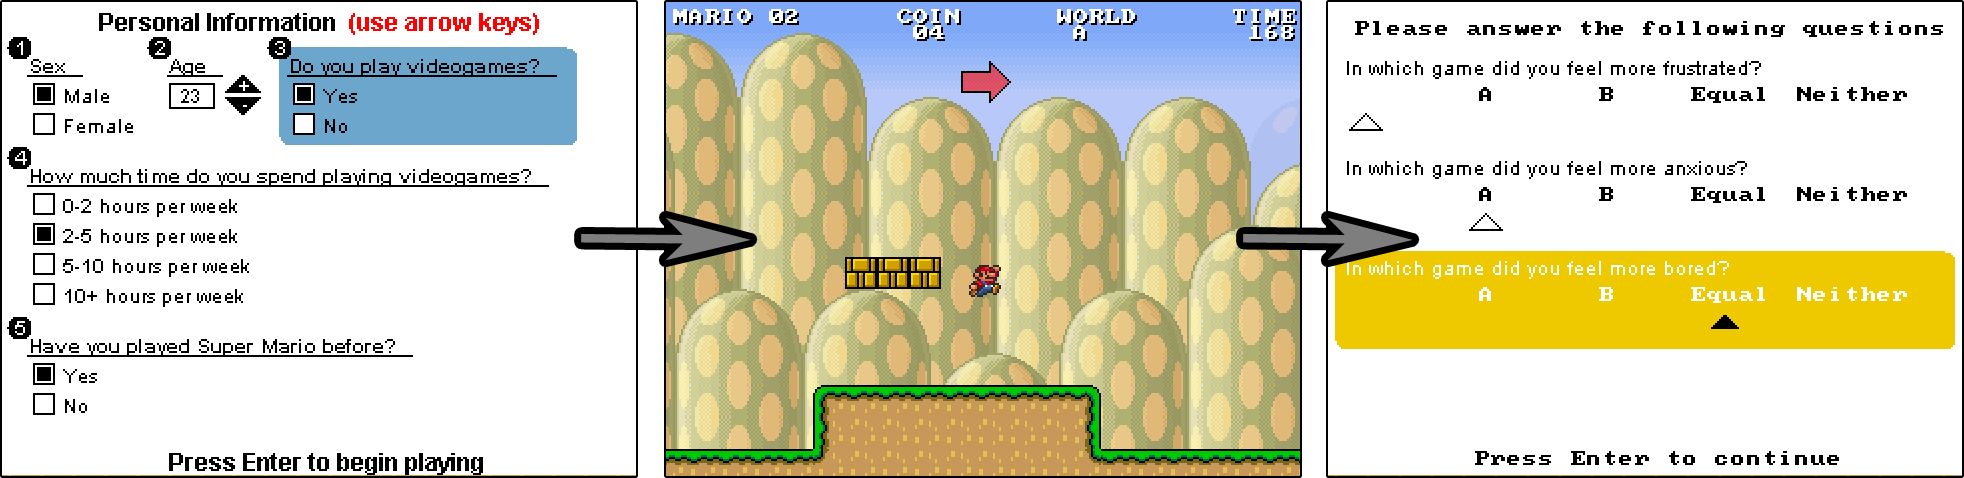
\includegraphics[width=0.95\textwidth]{Pics/mario_all2}
%\caption{Using a Java web applet, Pedersen, Togelius and Yannakakis collected data about player %preferences in level design, by building a questionnaire directly into the game. Figure inspired by %\cite{marioModel}.}
%\label{fig:mario}
%\end{figure*}
\section{Design \& Implementation} \label{design}
\subsection{Modulating Acceleration and Deceleration}
Swink discussed different ways to modulate the player avatar's movement in the chapter \textit{Response Metrics} \cite{swink}. Inspired by ADSR envelopes (Attack-Decay-Sustain-Release), Swink proposed the idea of using velocity modulation to change the game feel. Even if the input signal from the controller is discrete and binary (button is either pressed down or released), the software can modulate it into a continuous signal. By altering the attack and release phase (or, acceleration and deceleration), it is possible to create different game feel, as illustrated in Figures \ref{fig:adsr_stiff} and \ref{fig:adsr_loose}.

%, e.g., the sound of a pipe organ or a guitar string. This is achieved by modulating the amplitude over time.

%Inspired by Swink's discussion about \textit{Response Metrics} \cite{swink}, a 2D platforming game was developed. The game changes two types of parameters between each round: how fast the ball accelerates and how fast it decelerates when moving horizontally. Swink calls these the \textit{attack} and \textit{release} phases, or, the acceleration and deceleration of avatar movement. Hence, the velocity of the player's avatar is modulated over time, creating different types of game feel. Figures \ref{fig:adsr_stiff} and \ref{fig:adsr_loose} show two examples of the modulations proposed by Swink.


%According to Swink, when the acceleration or deceleration is very long (e.g., the avatar takes more than 100 milliseconds to be perceived to be moving), the impression of instantaneous response erodes. Even if there are small changes in the velocity, if these cannot be perceived by the player, the game might feel unresponsive \cite{swink}. This is illustrated by Figure \ref{fig:adsr}.

\begin{figure}[htbp]
\centering
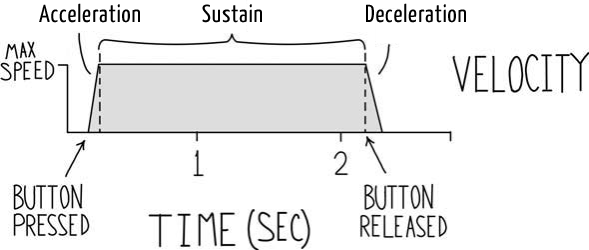
\includegraphics[width=0.30\textwidth]{Pics/adsr_stiff}
\caption{Short acceleration/deceleration gives a responsive, but stiff, feel. Figure inspired by Swink \cite{swink}.}
\label{fig:adsr_stiff}
\end{figure}

\begin{figure}[htbp]
\centering
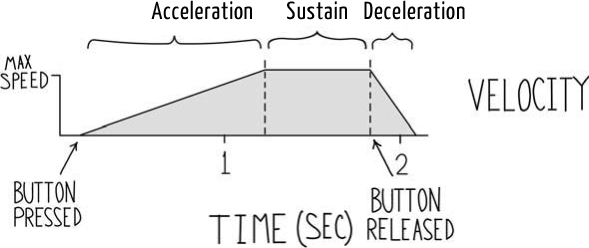
\includegraphics[width=0.30\textwidth]{Pics/adsr_loose}
\caption{Long acceleration gives a loose, but fluid, feel. Figure inspired by Swink \cite{swink}.}
\label{fig:adsr_loose}
\end{figure}

Taking inspiration from Swink, a 2D side-scrolling platformer game was developed in which players move a soccer ball from left to right to collect stars (see Figure \ref{fig:game}). The game is controlled with the keyboard. Similar to \textit{Super Mario Bros.}, there is a variable jump, meaning that holding down the button results in higher jumps.

Two parameters change between each round: how fast the ball accelerates and how fast it decelerates (when moving horizontally). Hence, the velocity of the player's avatar is modulated over time. This means that when the player presses the movement button, the ball takes a certain amount of time before it reaches its maximum velocity. The same is applied when the player releases the button: the ball gradually slows down, until it stops.

%To keep the experiment as simple as possible, only linear curves were considered for this project. Also, the decay phase was deemed unnecessary, since it wouldn't make sense for an avatar to accelerate, then decay a little, and then sustain the maximum velocity.

%Depending on how big a delay there is from the player triggering an event to getting feedback, the game will gradually feel less responsive.

Two intervals were chosen, inspired by Swink's model of player perception and feedback. The first interval, \textit{fast}, is between 1 millisecond and 240 milliseconds. The second interval, \textit{slow}, is from 241 milliseconds to 1500 milliseconds. For each round in the game, the player is assigned randomly-chosen values within the two intervals. 
%The reason for choosing random values instead of fixed values is that it isn't perfectly clear at which exact point a game goes from feeling responsive to unresponsive. Instead of choosing arbitrary fixed numbers, the system randomly assigns numbers within the two intervals. 
The acceleration/deceleration is thus scaled depending on the time values, using Equation \ref{eq:erl}.
\begin{equation} \label{eq:erl} %% source: http://www.calculatorsoup.com/calculators/physics/velocity_a_t.php
a = (v - v_0)/{\Delta}t
\end{equation} 
where $a$ is the acceleration/deceleration, $v$ is the target velocity, $v_0$ is the initial velocity and ${\Delta}t$ is the time after which the target velocity is reached.

%\begin{table} \centering
%\label{tab:time}
%\caption{Time intervals for the acceleration/deceleration.}
%\begin{tabular}{cc}
%\toprule
%\textbf{Fast} & \textbf{Slow} \\
%\midrule
%1 ms - 240 ms & 241 ms - 1500 ms\\
%\bottomrule
%\end{tabular}
%\end{table}

The game features other parameters, such as gravity, jump velocity and the aforementioned ``ghost jump", but only the horizontal ground acceleration and deceleration changed between rounds. Graphics and sound effects have been held to a minimum, since the influence of polishing effects is outside the scope of this project. Only a small trail renderer is attached to the ball. The ball also has a rolling animation that is linearly mapped to the horizontal velocity.

\begin{figure}[htbp]
\centering
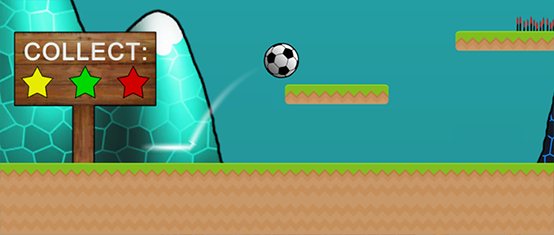
\includegraphics[width=0.3\textwidth]{Pics/gf}
\caption{Players control a rolling ball. Their task is to collect three stars.}
\label{fig:game}
\end{figure}

%Since the aim is to allow for players to experience the game feel as much as possible, the level has been designed to be simple and not too challenging, ensuring that most participants would complete the level without too much trouble.
%To ensure that all participants had comparable experiences, the game was fixed at a 960x600 resolution, no matter if played in a browser or as a standalone program. Also, the camera is set to follow the player avatar directly; however, small deadzones for vertical and horizontal movement were implemented, meaning that the camera will only move when the player moves outside these zones (e.g., by jumping more than a few pixels).
\section{Experimental Design} \label{experimentalDesign}
%\subsection{Research Question}
%How does the acceleration and deceleration of a player avatar influence the game feel of a 2D platformer? What types of words do players use to describe the game feeling, and what parameters result in these words?
%\subsection{Stimuli}
%The time it took for the player avatar to accelerate and decelerate changed between rounds.

\subsection{Stimulus Presentation}
Participants played four rounds of the game. Each round had different acceleration and deceleration values. All other factors were held constant, e.g., the level design, sound effects and the parameters for jumping. Between rounds, participants were asked to describe how it felt to play the game. The term \textit{game feel} was explicitly not explained, so that participants would try to describe the feel of the game from their own understanding of what game feel might be.

The experiment was designed as a repeated-measures, within-participant design \cite{cunningham}. This means that the participants were exposed to the stimuli (the changing acceleration and deceleration) multiple times. Additionally, each participant would see all of the available stimuli (each combination within the two categories, \textit{fast} and \textit{slow}), thereby acting as their own control group by comparing the different stimuli to each other.

\subsubsection{Latin Squares} \label{latinSection}
There are a total of four possible combinations, as is shown in Table \ref{tab:combinations}. One of the strengths with within-participant designs is that it doesn't require as many participants as a between-participant design, since each participant will try all the conditions. However, one disadvantage is the risk of carry-over effects \cite{experimental1}. This might be due to fatigue (e.g., participants becoming bored after having experienced the multiple conditions) or practice (e.g., participants are better at the end than when they started).

\begin{table} \centering
\caption{Four different combinations.}
\label{tab:combinations}
\begin{tabular}{ccc}
\toprule
& \textbf{Acceleration} & \textbf{Deceleration} \\
\midrule
\textbf{Stimulus 1} & Fast (A) & Fast (A)\\
\textbf{Stimulus 2} & Slow (B) & Slow (B)\\
\textbf{Stimulus 3} & Fast (A) & Slow (B)\\
\textbf{Stimulus 4} & Slow (B) & Fast (A)\\
\bottomrule
\end{tabular}
\end{table}

The order in which the different stimuli are shown can affect the participant's behaviour/perception. A way to prevent this is to use a counter-balanced design. This method reduces the risks of the order influencing the results \cite{experimental2}. Ideally, since there are four possible conditions, there should be 4x3x2x1 different orders, i.e., 24 orders of treatment. The number of participants must also be a multiple of 24, since there should be an equal number in each group \cite{experimental2}. Having 24 different combinations was deemed too complex; thus, an incomplete balanced design in the form of Latin squares was used instead (see Table \ref{table:latin}). Even though the order effects aren't eliminated completely, they become balanced.

\begin{table} \centering
\scriptsize
\caption{Latin squares are arranged in rows and columns such that each of the stimuli conditions only occur once in each row and column. The first letter is the acceleration, the second letter is the deceleration. `A' means fast and `B' means slow.}
\label{table:latin}
\begin{tabular}{ccccc}
\toprule
& \textbf{Stimulus 1} & \textbf{Stimulus 2} & \textbf{Stimulus 3} & \textbf{Stimulus 4}\\
\midrule
\textbf{Seq. 1} & AA & BB & BA & AB\\
\textbf{Seq. 2} & BB & AB & AA & BA\\
\textbf{Seq. 3} & AB & BA & BB & AA\\
\textbf{Seq. 4} & BA & AA & AB & BB\\
\bottomrule
\end{tabular}
\end{table}

\subsection{Task} \label{task}
In order to gather responses from the test participants, a questionnaire was built into the game. Initially, participants were asked to fill in basic demographical information. Before the game started, participants were unaware of what to expect: they didn't know the range of what stimuli they would see, hence, they might be hesitant to use the extreme values on the Likert scales in the questionnaire. To counter this, participants were presented with two examples of the conditions (very \textit{fast} and very \textit{slow} acceleration/deceleration) in a closed environment. This is called \textit{anchoring} \cite{cunningham} and gives participants a common reference point of what to expect in the game. However, the game doesn't explicitly describe the two examples, i.e., stating that it's the acceleration/deceleration that change.

%\begin{figure}[htbp]
%\centering
%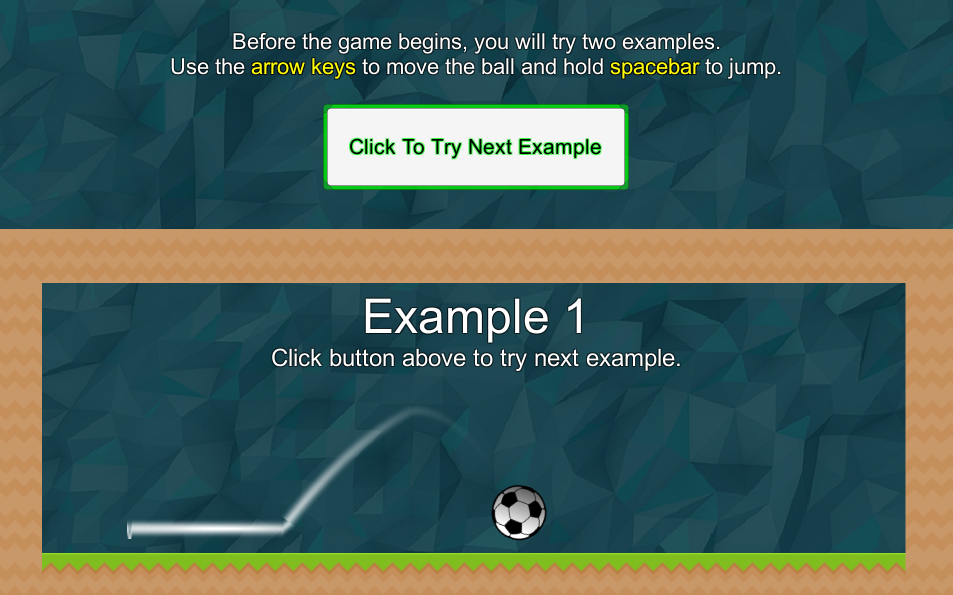
\includegraphics[width=0.4\textwidth]{Pics/example}
%\caption{Participants were shown two examples of the extreme conditions before playing the actual %game.}
%\label{fig:example}
%\end{figure}

Afterwards, the game begins and players are asked to find and collect three stars. The purpose of the stars is to ensure that players move/jump around enough in order to experience the feel of controlling the ball. The stars have been placed in the beginning, middle and end of the level, so players have to experience the whole level each time. The level consists of traditional platforming elements, as well as obstacles in the form of a few moving enemies and spikes. Figure \ref{fig:level} shows an overview of the game's level.

\begin{figure*}[htbp]
\centering
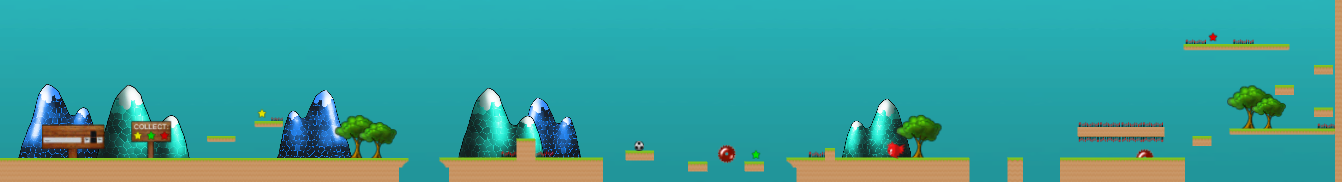
\includegraphics[width=1\textwidth]{Pics/levelStructure}
\caption{Participants played the same level four times.}
\label{fig:level}
\end{figure*}

Each time players collect three stars, the game is paused and a questionnaire is shown (see Figure \ref{fig:questionnaire}). The questionnaire consists of three sets of questions. The first asks players to try and describe the feeling of controlling the ball on the ground and in the air, with their own words. It is stressed that the chosen word(s) should be something that the player would use to describe the feeling to a friend. There were no restrictions on what types of words players could use (the input field's length is equivalent to approximately 66 characters, but it is possible to scroll forward/backward if a participant writes more than this). Each input field includes five randomly-chosen example words to give participants an idea of what could be used (see Table \ref{table:wordsExamples}). Participants were asked to describe the feeling both on the ground and in air. Even though only horizontal movement is changed in the form of the acceleration and deceleration (both apply on ground and in air), there is a possibility that players perceived the game feel differently on ground and in air. Instead of trying to describe both at the same time, players were shown two input fields.

\begin{table} \centering
\scriptsize
\caption{Participants were shown five randomly-chosen words to give them an idea of what they could write.}
\label{table:wordsExamples}
\begin{tabular}{ccccc}
\toprule
Fragile & Rigid & Firm & Solid & Thick\\
Fixed & Robust & Sore & Steadfast & Wild\\
Constant & Free & Hard & Tough & Restricted\\
Limited & Reduced & Fast & Heavy & Slow\\
Enjoyable & Stressful & Annoying & Realistic & Normal\\
Difficult & Easy & Dry & Juicy & Mechanical\\
Automatic & Organic & Exciting & Wet & Simple\\
Complicated & Direct & Inert & Unrealistic & Light\\
\bottomrule
\end{tabular}
\end{table}

After describing the game feel with the players' own words, a new set of questions was shown. Here, players were asked to rate the game feel on a 7-point Likert scale. Taking inspiration from Swink \cite{swink}, players rated the game feeling on how \textit{twitchy}, \textit{fluid}, \textit{stiff}, \textit{floaty} and \textit{responsive} they felt the controls were. Lastly, players were asked about how \textit{enjoyable}, \textit{difficult} and \textit{frustrating} it was to control the ball, as well as \textit{how much they liked} the control of the ball. In case players forgot how it felt to control the ball, they could always click on the \textit{Resume Playing} button to refresh their memories before continuing with the questionnaire.

After finishing the fourth round, participants were asked to complete an online post-questionnaire. The questions here were about game feel in general: \textit{What parameters do you think changed between each round in the ball game?} and \textit{In your own words, how would you define the feel of games?}.

\begin{figure*}[htbp]
\centering
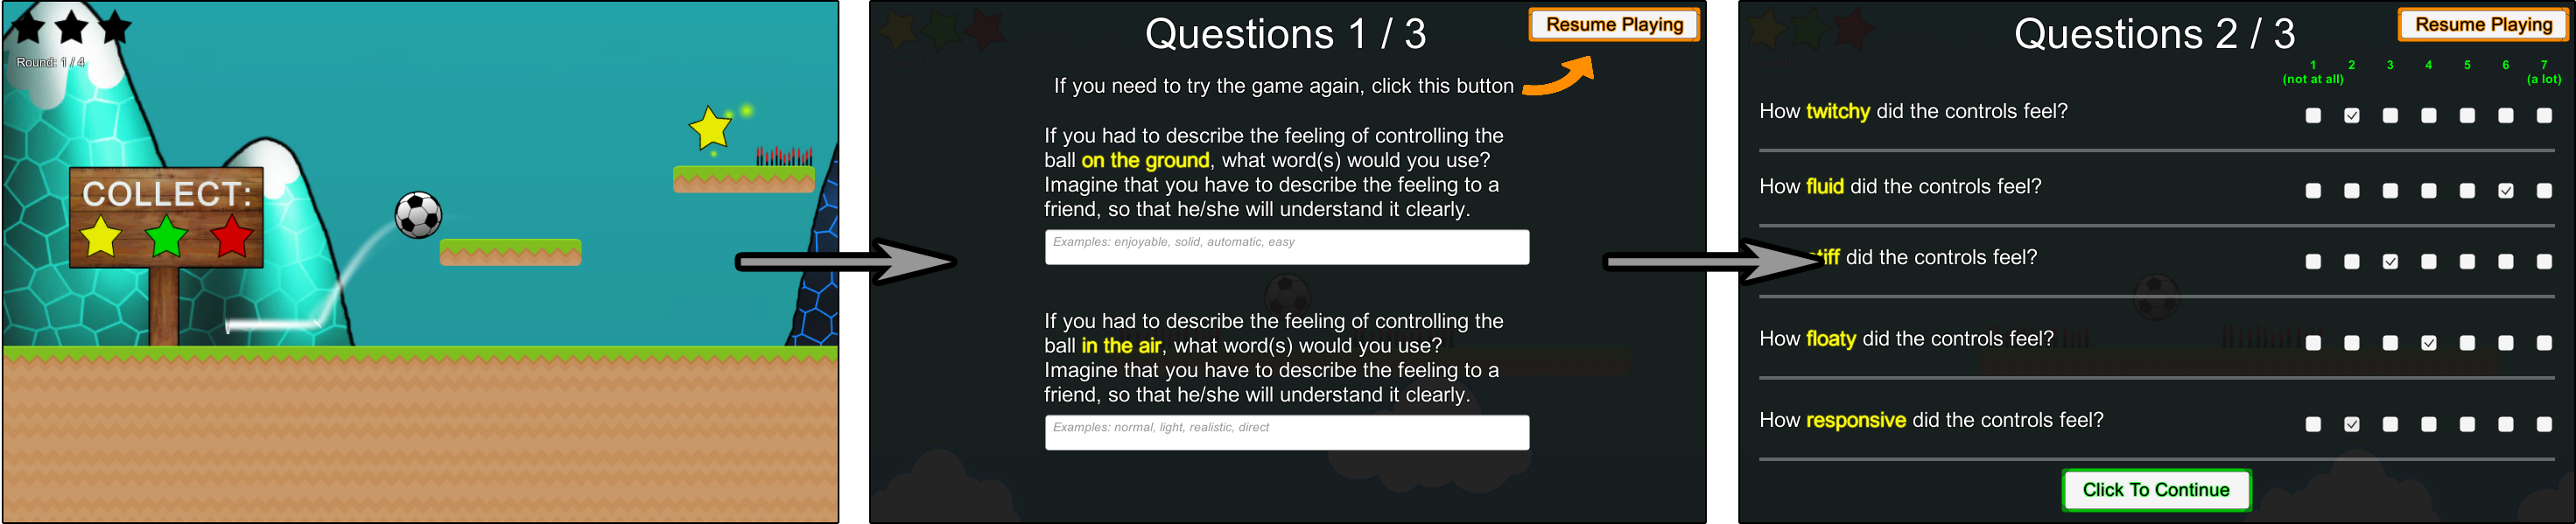
\includegraphics[width=0.95\textwidth]{Pics/game_phases}
\caption{When the player collected three stars, the game paused and showed a questionnaire.}
\label{fig:questionnaire}
\end{figure*}

\subsection{Participants}
The game was uploaded to a server and shared on social media websites and gaming forums. The primary target group was people who already play videogames; however, others were welcome to play the game as well. The participants were oblivious to the exact purpose and methods used in the experiment; they only knew that the research topic was about game feel (however, the term was never explained), but not how this was measured.

A landing page was created where participants could choose to either play the game in their browser or download a standalone build\footnote{The game is available here: \\ \url{http://tunnelvisiongames.com/g/GameFeel.html}}. Whenever a player completed a round (by collecting three stars and answering the questionnaire), data was sent to an MySQL database. The data entries included demographical information (age, gender, region, previous experience with games), parameter information (acceleration and deceleration times) and player descriptions (how players described the game feel, and how they rated the game feel on the pre-defined words). Target platform, player death count, average framerate and time spent on the level were also saved.
%To ensure the order in the Latin square (see Section \ref{latinSection}), players were assigned a number between 1 and 4 when starting the game. This number corresponds to the sequences in Table \ref{table:latin}. This was achieved by taking modulus 4 of the total amount of participants having completed the experiment and adding 1 to it. For instance, if 26 participants had played the game before entering, the next player would be assigned the sequence number (26 \% 4) + 1 = 3.
\section{Data Analysis} \label{data}
The data is split into three main parts: \textit{demographics} (before playing the game), \textit{mid-questionnaire} (while playing the game) and \textit{post-questionnaire} (after playing the game). The mid-questionnaire consists of two parts. In the first part, participants describe the game feel in their own words. In the second part, participants rate the game feel on pre-defined words using Likert scales. The post-questionnaire is about game feel in general. The following analyzes the data from the three parts.

\subsection{Demographics}
As stated previously, the game was mainly shared on gaming websites. At the time of writing, 274 participants have played the game. Tables \ref{table:demographics1} and \ref{table:demographics2} show demographical data about the participants. Most of the participants rated themselves rather experienced with both playing videogames in general and playing 2D platforming games. The average framerate for all participants was 59.7 FPS, and the average time spent per level was 61 seconds/level.

\begin{table} \centering
\small
\caption{Demographics data 1.}
\label{table:demographics1}
\renewcommand{\arraystretch}{1.2}
\begin{tabular}{cccc}
\midrule
\textbf{Platform} & Windows Web: & Windows Exe: & Mac Web: \\
                  & 55.2\%      & 30.7\%      & 14.1\%  \\
\textbf{Gender}   & Male:        & Female:      & Other:   \\
                  & 93.6\%      & 5.7\%       & 0.7\%   \\
\textbf{Age}      & Male:     & Female:            & Other:        \\
                  & 24.6 years  & 23.9 years           & 25 years        \\
\bottomrule
\end{tabular}
\end{table}

\begin{table} \centering
\small
\caption{Demographics data 2.}
\label{table:demographics2}
%\renewcommand{\arraystretch}{1.2}
\begin{tabular}{lcc}
\midrule
\textbf{Regions}                      &                & \textbf{}               \\ 
\textit{Europe}                      & 70.6\%         &                         \\
\textit{Americas}                    & 26.7\%         &                         \\
\textit{Asia}                        & 1.9\%          &                         \\
\textit{Oceania}                     & 0\%            &                         \\
\textit{Africa}                      & 0.6\%          &                         \\
\textit{Other}                       & 0.2\%          &                         \\
\textbf{Experience with...} & \textbf{Videogames} & \textbf{2D platformers} \\
\textit{1 (none)}                           & 0\%            & 0\%                     \\
\textit{2}                           & 0\%            & 3.1\%                   \\ 
\textit{3}                           & 0.6\%          & 10.1\%                  \\
\textit{4}                           & 4\%            & 14.1\%                  \\ 
\textit{5}                           & 9.6\%          & 23.2\%                  \\ 
\textit{6}                           & 22.5\%         & 16.9\%                  \\
\textit{7 (a lot)}                           & 63.3\%         & 32.6\%                  \\
\bottomrule
\end{tabular}
\end{table}

As stated in Section \ref{latinSection}, ideally there should be an equal amount of participants in each of the four Latin square sequences. However, as shown in Table \ref{table:latinSequenceNumber}, this is not the case. This might be due to either players quitting halfway, or that participants for some reason lost the Internet connection while trying to access the current Latin square number (in this case, the sequence was chosen randomly). Each time a participant collects three stars and answers the mid-questionnaire, data is logged. In total, 701 data logs were collected. Figure \ref{fig:retention} illustrates the retention rate of the participants.

\begin{table} \centering
%\small
\caption{The number of participants in each of the four Latin square sequences.}
\label{table:latinSequenceNumber}
\begin{tabular}{cc}
\toprule
& \textbf{Number of participants}\\
\midrule
\textbf{Sequence 1} & 190\\
\textbf{Sequence 2} & 179\\
\textbf{Sequence 3} & 165\\
\textbf{Sequence 4} & 167\\
\bottomrule
\end{tabular}
\end{table}

\begin{figure}[htbp]
\centering
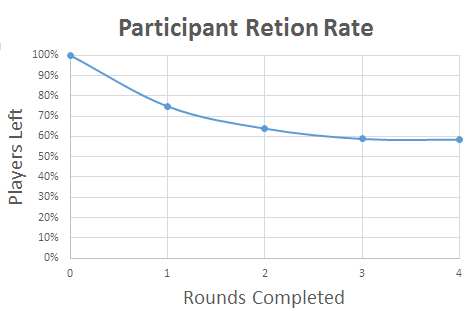
\includegraphics[width=0.4\textwidth]{Pics/retetionRate}
\caption{274 participants started the game, but not all completed the four rounds, presumably due to fatigue or boredom.}
\label{fig:retention}
\end{figure}

\subsection{Mid-questionnaire}
Whenever players collected three stars, they were met with a set of questions (see Figure \ref{fig:questionnaire}). In the first part, participants describe the game feel in their own words, while in the second part they rate pre-defined words on a 7-point Likert scale (1 = \textit{not at all}; 7 = \textit{a lot}).

\subsubsection{Describing Game Feel in Own Words}
To get an overview of the words participants used, a word cloud has been generated (see Figure \ref{fig:wordcloud}). This illustrates the most commonly-used words, such as \textit{ball}, \textit{control}, \textit{fast}, \textit{heavy}, \textit{slow}, \textit{like}, \textit{responsive}, \textit{sluggish}, \textit{easy} and \textit{momentum}.

The words that the participants used to describe the game feel have manually, by a the author, been put into one or more of following nine categories (see Figure \ref{fig:coding1}). Note that a description can include words from multiple categories at once. The average word count for ground descriptions is 5,4 words.
\begin{itemize}[noitemsep,nolistsep]
\item Single words or multiple words?
\item Basic or complex words (basic words are root words that can stand on their own, e.g., \textit{heavy} and \textit{laggy}, whereas complex words consist of modifiers that somehow change the meaning of the root words, e.g., \textit{very fast} or \textit{a bit sluggish})?
\item Did the words describe a quality/opinion (using words such as \textit{fun}, \textit{too fast} or \textit{very annoying} or \textit{unrealistic})?
\item Did the words describe anything related to the difficulty; did the words use physical properties (\textit{like dragging through light mud}, using words such as \textit{force} and \textit{momentum})?
\item Did the words make comparisons to other games (\textit{like Mario} or \textit{like Mega Man})?
\item Did the words make comparisons to previous rounds of the game (\textit{similar to last round})?
\end{itemize}

\begin{figure}[htbp]
\centering
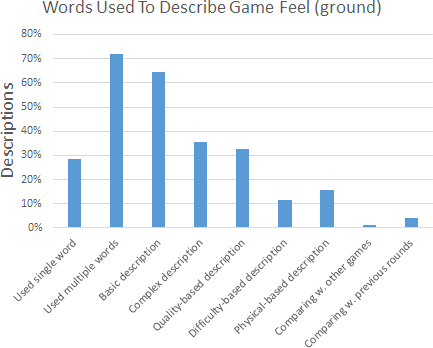
\includegraphics[width=\columnwidth]{Pics/coding1}
\caption{Coding1. NOTE: Coding not done yet.}
\label{fig:coding1}
\end{figure}

\begin{figure*}[htbp]
\centering
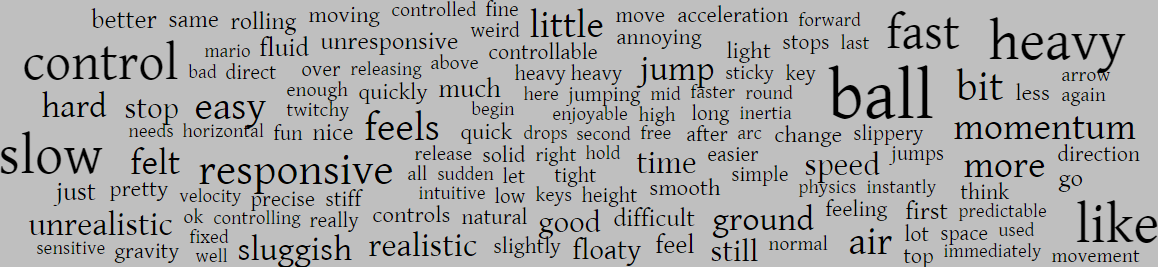
\includegraphics[width=1\textwidth]{Pics/wordcloud}
\caption{The 130 most commonly-used words to describe the feel of the controls (both on ground and in air). Bigger means a word has been used more frequently. Common words such as \textit{a}, \textit{also}, \textit{and}, \textit{have}, \textit{could}, etc. have been excluded. Created with WordItOut.com.}
\label{fig:wordcloud}
\end{figure*}

\subsubsection{Rating Game Feel with Pre-Defined Words}
Using a 7-point Likert scale, participants rated the game feel on the following pre-defined words.
\begin{itemize}[noitemsep,nolistsep]
\item Twitchy
\item Fluid
\item Stiff
\item Floaty
\item Responsive
\item Enjoyable
\item Difficult
\item How much they liked the controls
\item Frustration
\end{itemize}

%\begin{figure}[htbp]
%\centering
%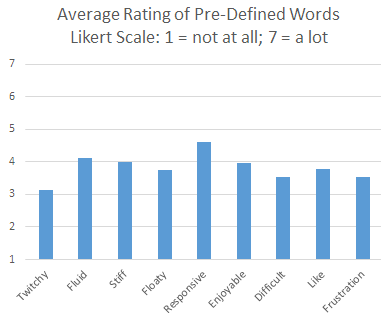
\includegraphics[width=0.35\textwidth]{Pics/average_rating}
%\caption{Averages of how participants rated the game feel across the pre-defined words.}
%\label{fig:average_rating}
%\end{figure}

One way to illustrate the responses is to plot the average ratings using acceleration and deceleration times, respectively (see Figures \ref{fig:acc_average_response} and \ref{fig:dec_average_response}). Even though one might be able to spot some slight tendencies, this way of showing the data is not accurate, since it splits up the acceleration and deceleration. The participants did not experience either in a vacuum; both were apparent all the time.

\begin{figure}[htbp]
\centering
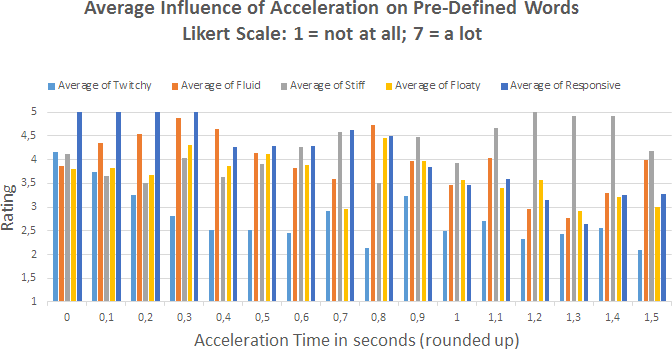
\includegraphics[width=0.97\columnwidth]{Pics/acc_average_response}
\caption{Average ratings with acceleration.}
\label{fig:acc_average_response}
\end{figure}

\begin{figure}[htbp]
\centering
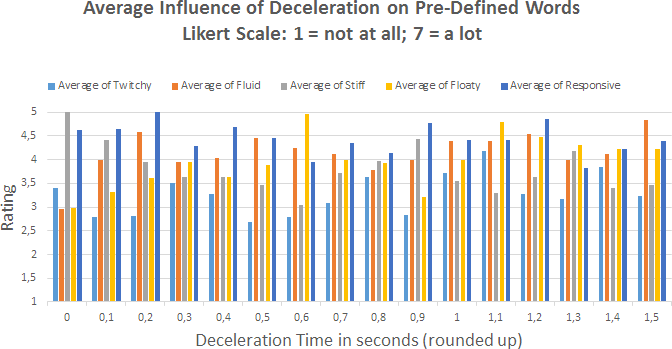
\includegraphics[width=0.97\columnwidth]{Pics/dec_average_response}
\caption{Average ratings with deceleration.}
\label{fig:dec_average_response}
\end{figure}

A different way to plot the data is to use both acceleration and deceleration at the same time. The following graphs show how the participants rated the game across the different words. For the case of clarity, only answers 1, 4 and 7 on the Likert scale are shown. Looking at the data, it appears as if the perceived contribution of the acceleration and deceleration times, respectively, aren't always equal.

When looking at Figure \ref{fig:twitchy}, it seems like the acceleration have a bigger influence than the deceleration when it comes to how \textit{twitchy} the game felt. Even with relatively high deceleration times (> 1 second), some participants still rated the game to feel very twitchy.

Figure \ref{fig:fluid} shows how \textit{fluid} participants perceived the game. Again, it is difficult to find a strong pattern, since participants with both small (< 0.4 seconds) and high (> 0.6 seconds) acceleration/deceleration times report the game to feel relatively fluid. However, it is clear that high acceleration time (> 0.6 seconds) results in a perception of low fluid.

With \textit{stiffness}, it appears that the deceleration has a greater influence than acceleration. This is evident in Figure \ref{fig:stiff}. Even with high acceleration times (> 0.6 seconds), participants still reported the game to feel stiff, as long as the deceleration time was below about 0.4 seconds.

Figure \ref{fig:floaty} shows a slight tendency towards high deceleration times (> 1 second) for a more \textit{floaty} feel. That being said, many reported gave the rating 4 around deceleration time 0.2 seconds.

With \textit{responsiveness}, there is a clear tendency towards acceleration having a bigger influence than deceleration. It seems like acceleration times below 0.2 seconds makes the game feel responsive. Likewise, when it comes to \textit{frustration}, Figure \ref{fig:frustration} shows that acceleration and deceleration times above 0.2 seconds makes participant feel frustration.

%width=\columnwidth
\begin{figure*}[htbp]
\centering
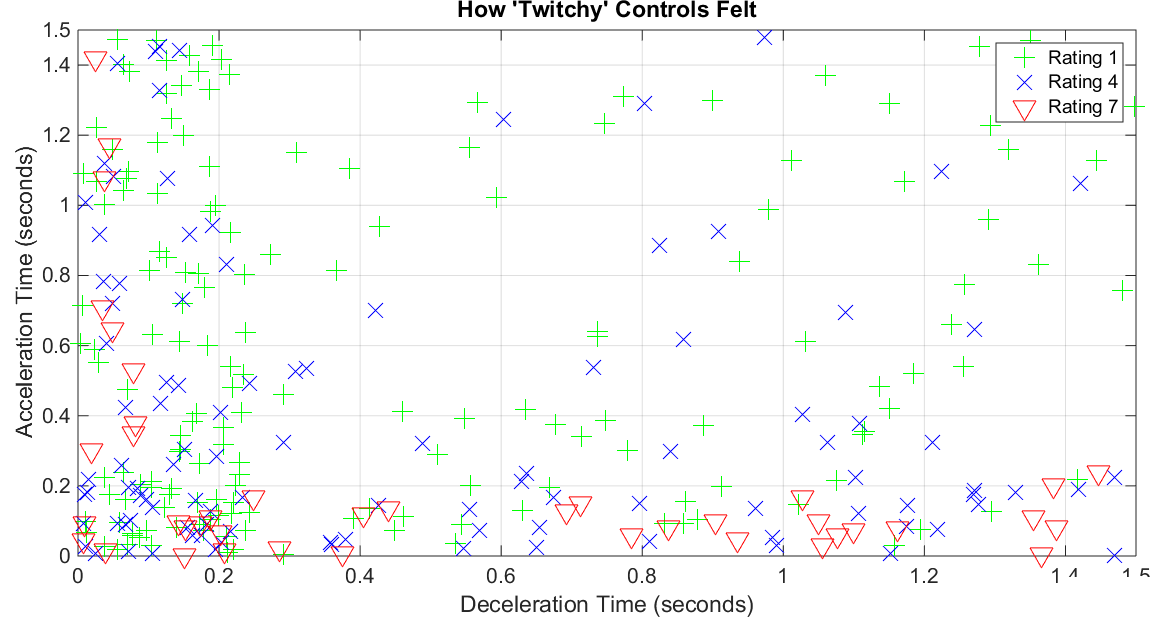
\includegraphics[width=0.67\textwidth]{Pics/Classes/Twitchy_classes}
\caption{Players' self-reported perception on how twitchy the controls felt, rated using a 7-point Likert scale (only 1, 4 and 7 are shown).}
\label{fig:twitchy}
\end{figure*}

\begin{figure*}[htbp]
\centering
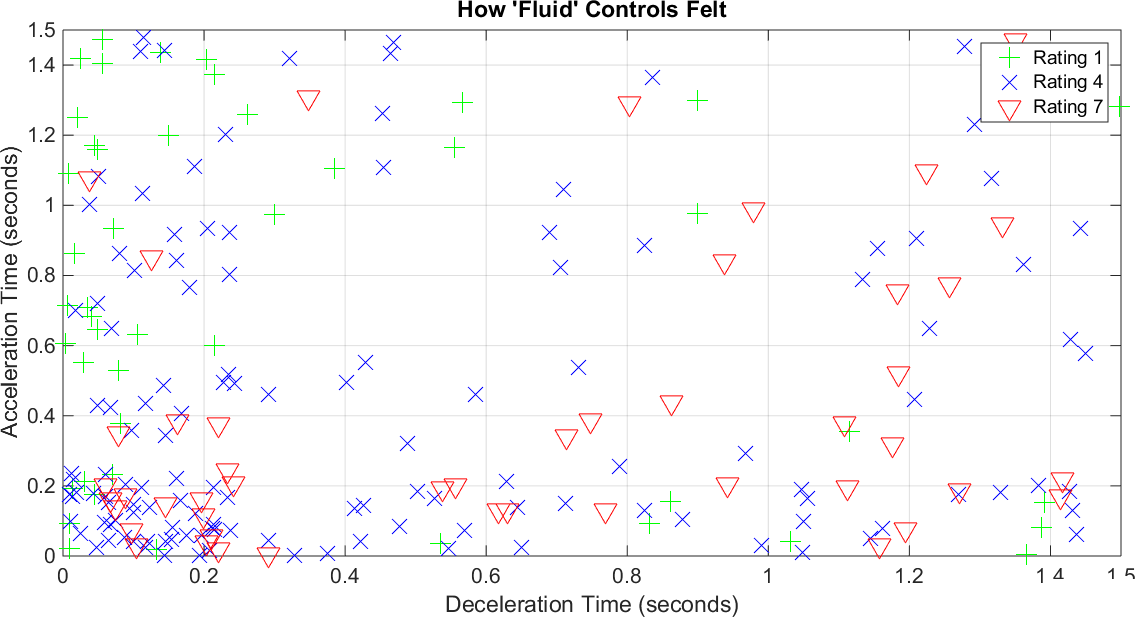
\includegraphics[width=0.67\textwidth]{Pics/Classes/Fluid_classes}
\caption{Players' self-reported perception on how fluid the controls felt, rated using a 7-point Likert scale (only 1, 4 and 7 are shown).}
\label{fig:fluid}
\end{figure*}

\begin{figure*}[htbp]
\centering
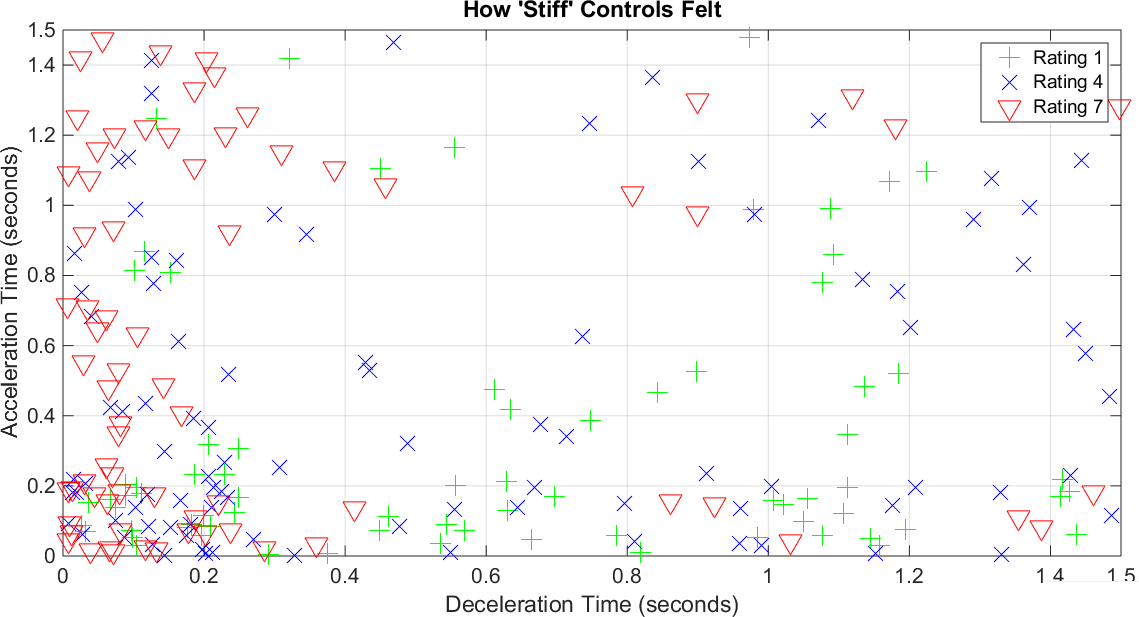
\includegraphics[width=0.67\textwidth]{Pics/Classes/Stiff_classes}
\caption{Players' self-reported perception on how stiff the controls felt, rated using a 7-point Likert scale (only 1, 4 and 7 are shown).}
\label{fig:stiff}
\end{figure*}

\begin{figure*}[htbp]
\centering
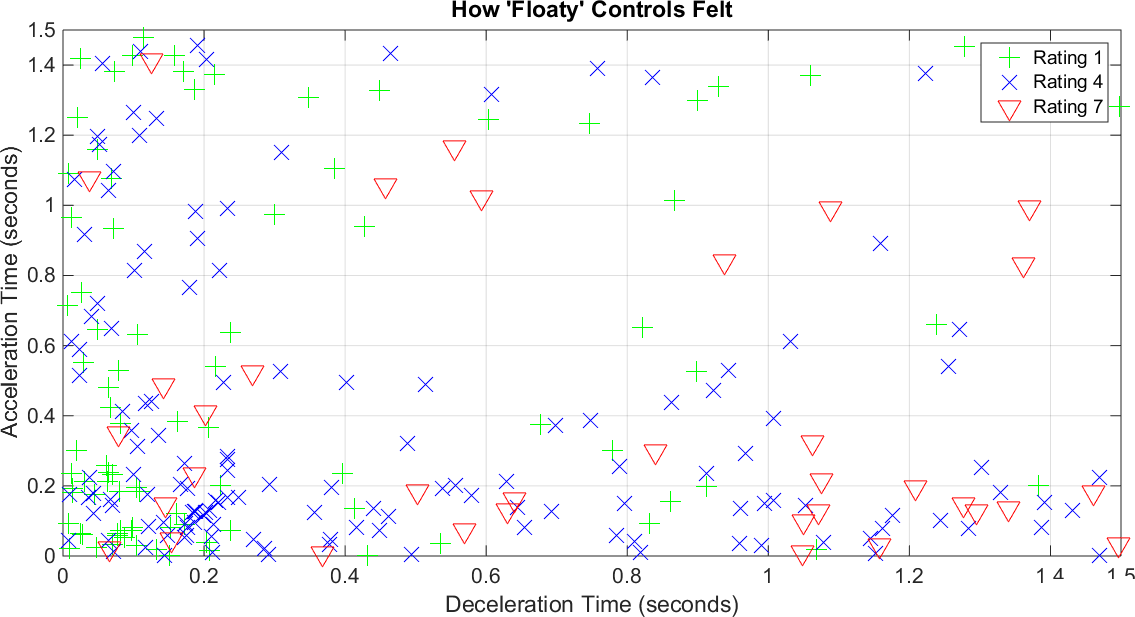
\includegraphics[width=0.67\textwidth]{Pics/Classes/Floaty_classes}
\caption{Players' self-reported perception on how floaty the controls felt, rated using a 7-point Likert scale (only 1, 4 and 7 are shown).}
\label{fig:floaty}
\end{figure*}

\begin{figure*}[htbp]
\centering
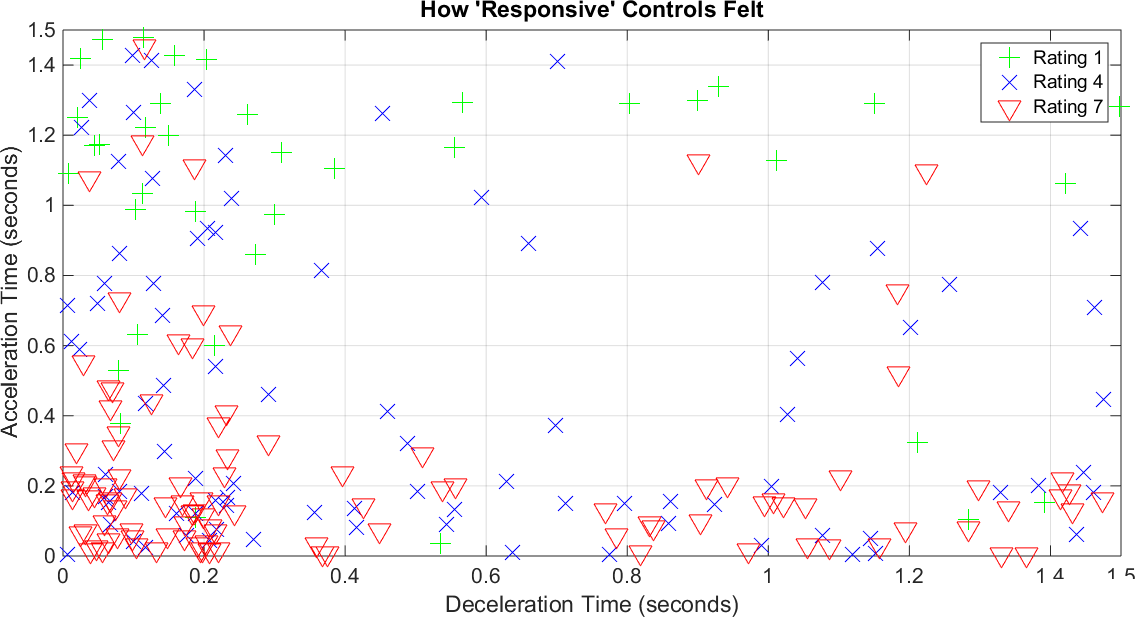
\includegraphics[width=0.67\textwidth]{Pics/Classes/Responsive_classes}
\caption{Players' self-reported perception on how responsive the controls felt, rated using a 7-point Likert scale (only 1, 4 and 7 are shown).}
\label{fig:responsive}
\end{figure*}

\begin{figure*}[htbp]
\centering
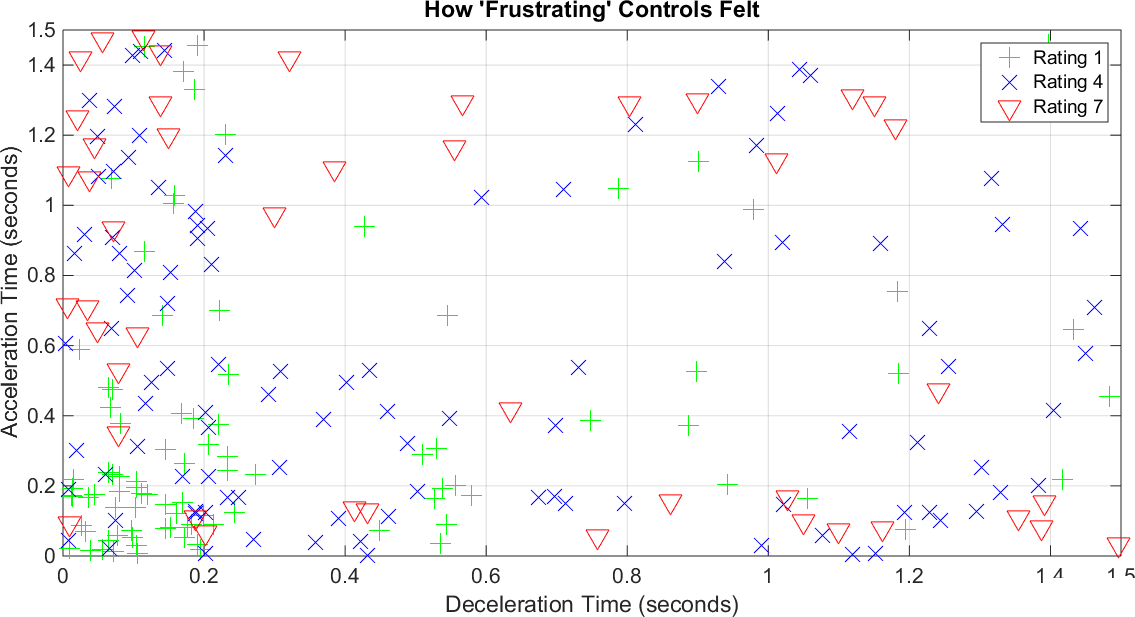
\includegraphics[width=0.67\textwidth]{Pics/Classes/Frustration_classes}
\caption{Players' self-reported perception on how frustrating the controls felt, rated using a 7-point Likert scale (only 1, 4 and 7 are shown).}
\label{fig:frustration}
\end{figure*}

A different way to visualize the data is to take the averages of the acceleration/deceleration times for each of the ratings, e.g., what are the average acceleration/deceleration times for twitchy rating 1, rating 2, rating 3, etc. However, since a Likert scale consists of ordinal values, there is no guarantee that a rating difference of e.g. 1 represents an equal conceptual change, since the scale might be used differently by different participants. For instance, some participants might be hesitant to use the extreme values 1 (not at all) and 7 (a lot), while others might spread their answers across the whole scale \cite{cunningham}. Because of this, in the following graphs, the averages have been put into three weighted categories, so that the extreme ends contribute more. The \textit{low rating} curve consists of ratings 1 (70\%), 2 (20\%) and 3 (10\%). The \textit{mid rating} curve consists of ratings 3 (25\%), 4 (50\%) and 5 (25\%). The \textit{high rating} consists of ratings 5 (10\%), 6 (20\%) and 7 (70\%). Using these numbers, it is now possible to draw attack/deceleration curves (see Figures \ref{fig:curve_twitchy}, \ref{fig:curve_fluid}, \ref{fig:curve_stiff}, \ref{fig:curve_floaty} and \ref{fig:curve_floaty}). For all curves, the sustain time is 1 second. The numbers in square brackets represent acceleration and deceleration times.

At first glance, most of the curves seem similar. However, when comparing the three curves from the same word, there are some differences. For instance, there is a difference of about 360 milliseconds between the deceleration time in \textit{low rating} and \textit{high rating} in the \textit{floaty}. curve. Also, it should be noted that the difference words are not mutually exclusive, i.e., the controls can feel floaty and fluid at the same time.

\begin{figure}[htbp]
\centering
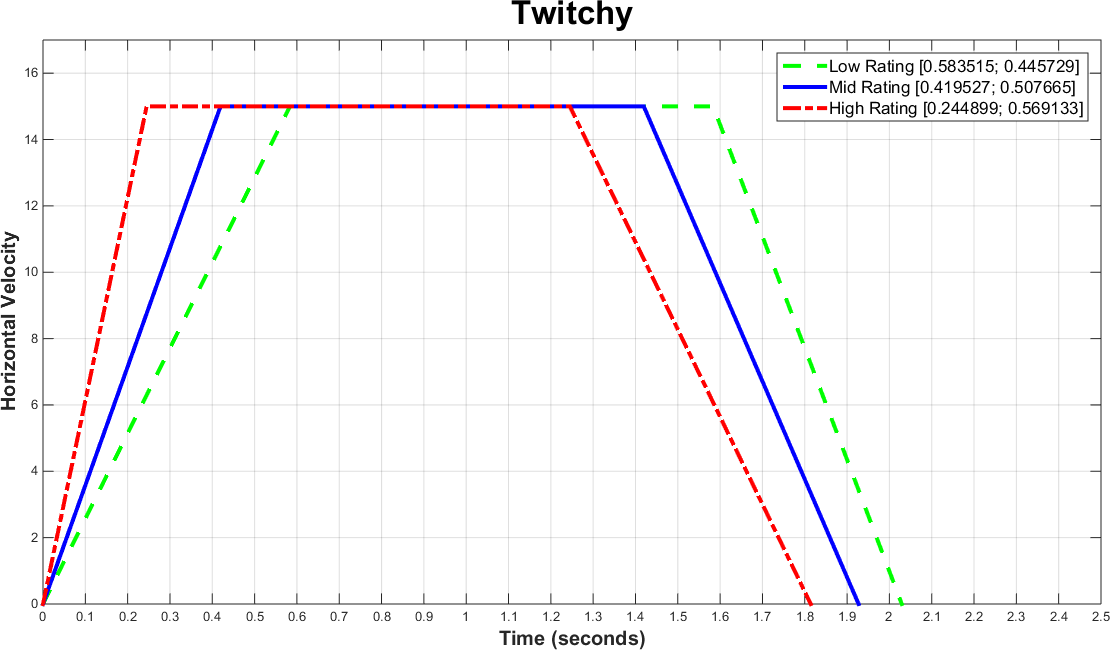
\includegraphics[width=0.9\columnwidth]{Pics/Curves/Twitchy_curve}
\caption{Average curves of twitchy controls.}
\label{fig:curve_twitchy}
\end{figure}

\begin{figure}[htbp]
\centering
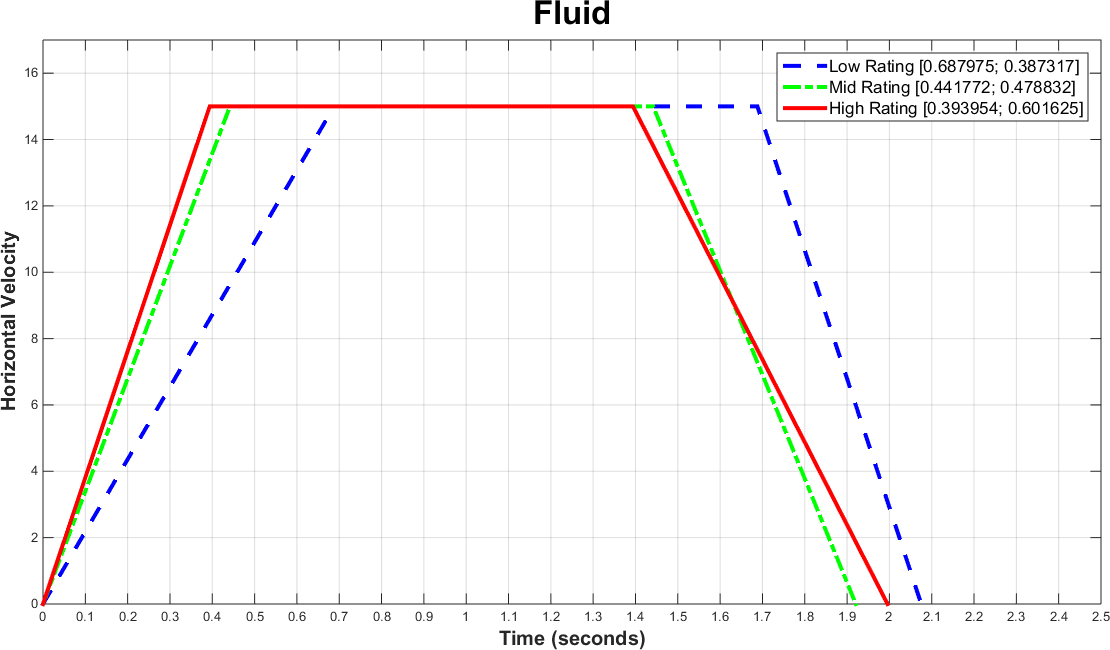
\includegraphics[width=0.9\columnwidth]{Pics/Curves/Fluid_curve}
\caption{Average curves of fluid controls.}
\label{fig:curve_fluid}
\end{figure}

\begin{figure}[htbp]
\centering
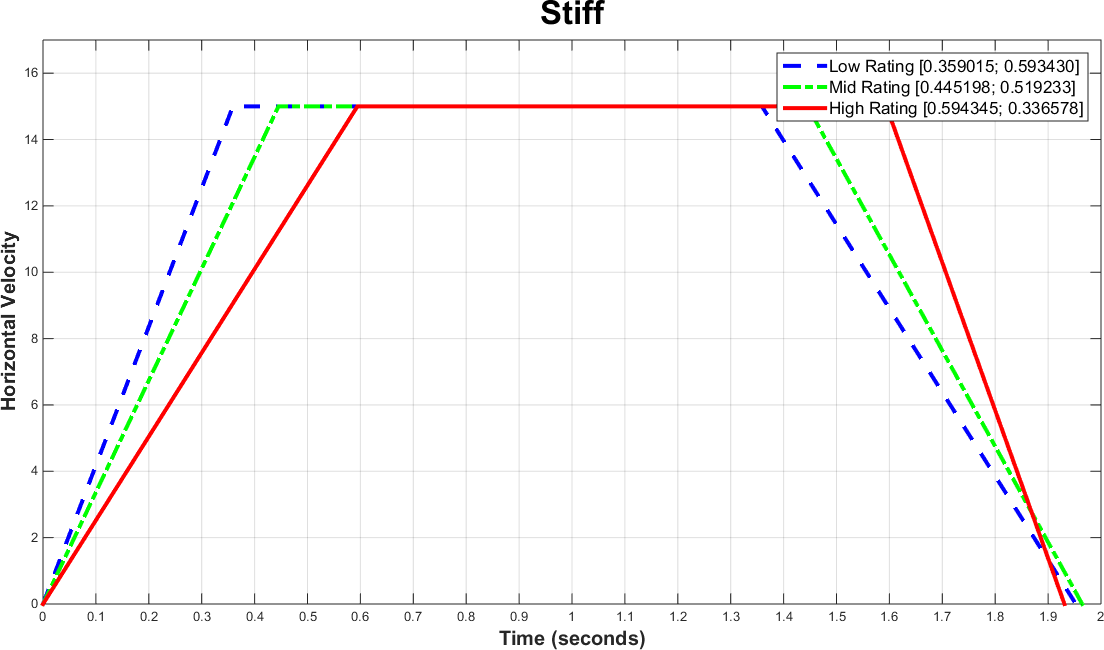
\includegraphics[width=0.9\columnwidth]{Pics/Curves/Stiff_curve}
\caption{Average curves of stiff controls.}
\label{fig:curve_stiff}
\end{figure}

\begin{figure}[htbp]
\centering
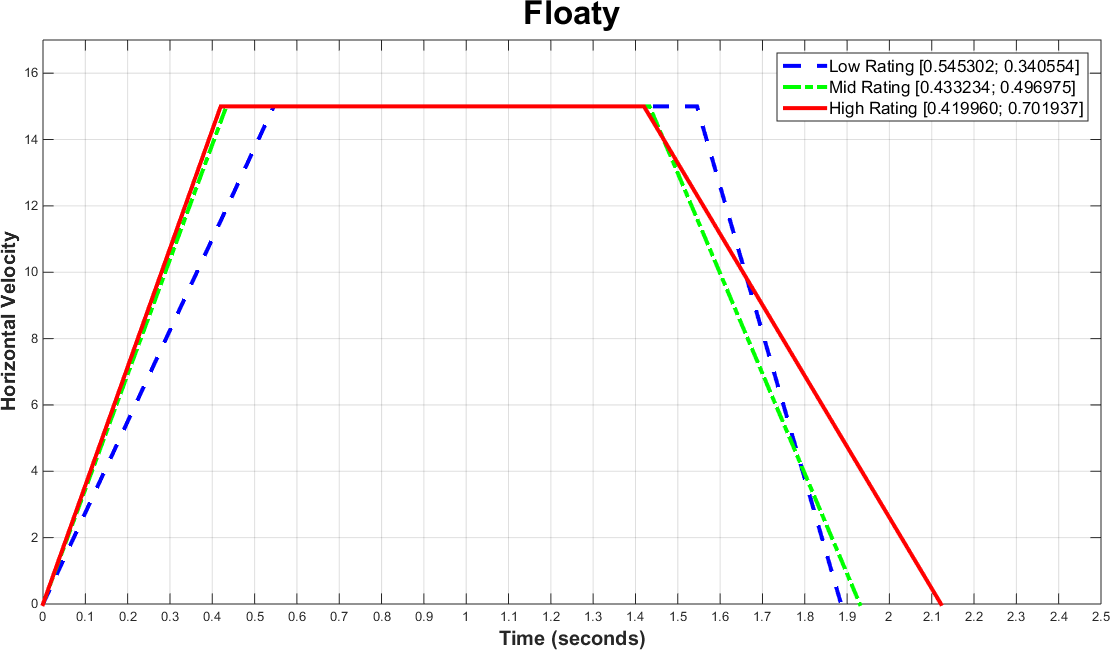
\includegraphics[width=0.9\columnwidth]{Pics/Curves/Floaty_curve}
\caption{Average curves of floaty controls.}
\label{fig:curve_floaty}
\end{figure}

\begin{figure}[htbp]
\centering
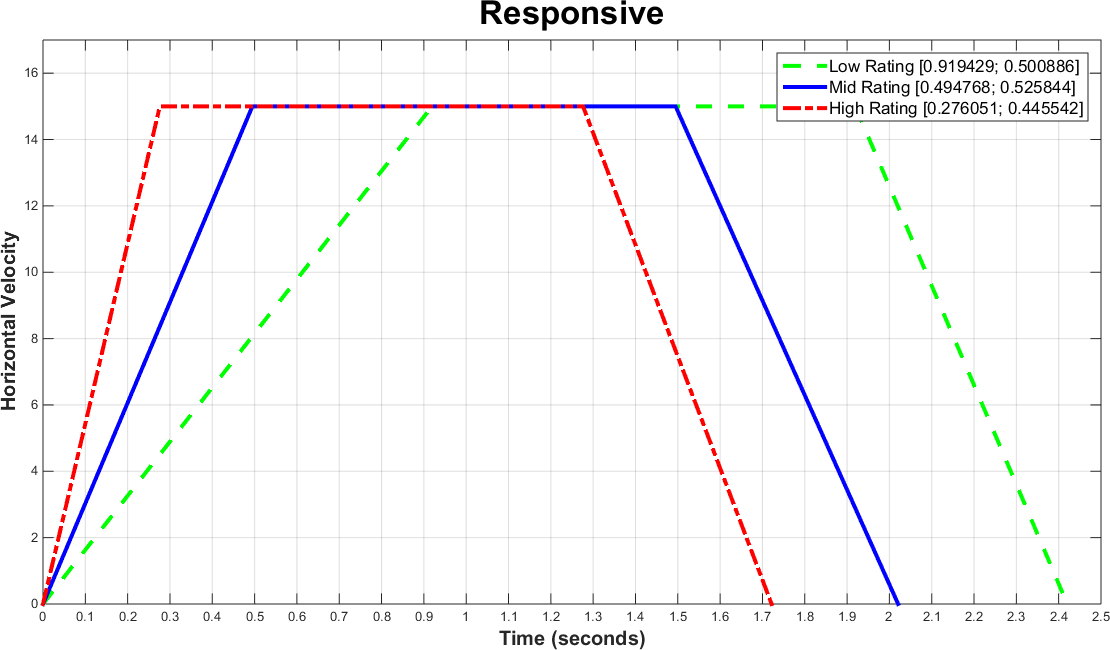
\includegraphics[width=0.9\columnwidth]{Pics/Curves/Responsive_curve}
\caption{Average curves of responsive controls.}
\label{fig:curve_responsive}
\end{figure}

\subsection{Post-questionnaire}
When completing the fourth round of the game, a link was shown to a Google Forms questionnaire. At the time of writing, 146 participants have taken part in this post-questionnaire.
\section{Discussion \& Conclusion} \label{discussion}
When it comes to how people describe game feel in their own words, it seems that many use basic descriptions such as `heavy', `slow', `responsive', `realistic', `sluggish' and `floaty'. For this type of game those description might be enough to describe the game feel.

There are a few correlations between the acceleration, deceleration and the pre-defined words. However, it seems like there are different interpretations of what those words mean, e.g., what it means for a game to feel \textit{stiff}.

While some participants seemed quite sensitive to even smaller changes, others reported that they didn't feel any difference between the rounds.

The curves presented in this paper are based on averages. The results are less clear-cut when compared to those provided by Swink (see Section \ref{design}). In this experiment, participants were asked to rate the acceleration and deceleration values along a group of Likert scales. An alternative approach would be to use A/B testing and ask participants whether stimulus A felt more or less \textit{twitchy} than stimulus B. It would also be interesting to let players themselves tweak and tune the game's parameters in order to achieve what they think feels best.

Furthermore, one could look into more evenly-distributed sequences of the stimuli, say, within the 240 ms interval. Also, it might be interesting to look into non-linear curves and the influence of how responsive this feels (e.g., a slow acceleration that starts with an initial bump in its curve).

It appears that some participants were confused by the term \textit{game feel}. This is to be expected, since it's still a loose and relatively unknown concept about how players perceive games. A similar term, \textit{mouthfeel}, describes, as the name suggests, the sensation of food in the mouth. Even though the term was coined in 1951 \cite{mouthfeel}, it is still a relatively unknown concept. It might take a while before game feel finds its place in the vocabulary of the common game player.

Game feel is a holistic experience with many contributing factors. In this experiment, only the avatar movement was looked at. However, all other elements still indirectly influence the overall game feel, such as the rolling animation of the ball; the gravity and jumping mechanic; the level design; and the input device. It is unclear how big an influence the altering acceleration/deceleration has over these other factors, as well as other contributing elements such as the attention, mood and motivation of the player. Further research into the influence of these is required.

\bibliographystyle{abbrv}
\begin{verbatim}

\end{verbatim}
\bibliography{references}  % sigproc.bib is the name of the Bibliography in this case

\balancecolumns
% That's all folks!
\end{document}
